\documentclass[aps,prl,twocolumn,groupedaddress]{revtex4-1}
% \documentclass[aps,twocolumn,secnumarabic,balancelastpage,amsmath,amssymb,nofootinbib]{revtex4-1}
\usepackage{amsmath}
\usepackage{amssymb}
\usepackage{amsfonts}
\usepackage{chapterbib}
\usepackage{color}
\usepackage{graphics}
\usepackage[pdftex]{graphicx}
\usepackage{grffile}
\usepackage{longtable}
\usepackage{epsf}
\usepackage{bm}
\usepackage{tikz}
\usepackage{asymptote}
\usepackage{thumbpdf}
\usepackage{bbm}
\usepackage{amscd}
\usepackage{units}
\usepackage{textcomp}
\usepackage[utf8x]{inputenc}
\usepackage{feyn}
\usepackage{feynmp}
\usepackage[colorlinks=true]{hyperref}
\newcommand{\drelectron}[1]{\node at #1 [circle, draw, inner sep=0pt, minimum size=1pt] {\_}}

\newcommand{\ud}{\mathrm{d}}
\newcommand{\ue}{\mathrm{e}}
\newcommand{\ui}{\mathrm{i}}
\newcommand{\res}{\mathrm{Res}}
\newcommand{\Tr}{\mathrm{Tr}}
\newcommand{\dsum}{\displaystyle\sum}
\newcommand{\dprod}{\displaystyle\prod}
\newcommand{\dlim}{\displaystyle\lim}
\newcommand{\dint}{\displaystyle\int}
\newcommand{\fsno}[1]{{\!\not\!{#1}}}
\newcommand{\eqar}[1]
{
  \begin{align*}
    #1
  \end{align*}
}
\newcommand{\eqarn}[1]
{
  \begin{align}
    #1
  \end{align}
}
\newcommand{\texp}[2]{\ensuremath{{#1}\times10^{#2}}}
\newcommand{\dexp}[2]{\ensuremath{{#1}\cdot10^{#2}}}
\newcommand{\eval}[2]{{\left.{#1}\right|_{#2}}}
\newcommand{\paren}[1]{{\left({#1}\right)}}
\newcommand{\lparen}[1]{{\left({#1}\right.}}
\newcommand{\rparen}[1]{{\left.{#1}\right)}}
\newcommand{\abs}[1]{{\left|{#1}\right|}}
\newcommand{\sqr}[1]{{\left[{#1}\right]}}
\newcommand{\crly}[1]{{\left\{{#1}\right\}}}
\newcommand{\angl}[1]{{\left\langle{#1}\right\rangle}}
\newcommand{\tpdiff}[4][{}]{{\paren{\frac{\partial^{#1} {#2}}{\partial {#3}{}^{#1}}}_{#4}}}
\newcommand{\tpsdiff}[4][{}]{{\paren{\frac{\partial^{#1}}{\partial {#3}{}^{#1}}{#2}}_{#4}}}
\newcommand{\pdiff}[3][{}]{{\frac{\partial^{#1} {#2}}{\partial {#3}{}^{#1}}}}
\newcommand{\diff}[3][{}]{{\frac{\ud^{#1} {#2}}{\ud {#3}{}^{#1}}}}
\newcommand{\psdiff}[3][{}]{{\frac{\partial^{#1}}{\partial {#3}{}^{#1}} {#2}}}
\newcommand{\sdiff}[3][{}]{{\frac{\ud^{#1}}{\ud {#3}{}^{#1}} {#2}}}
\newcommand{\tpddiff}[4][{}]{{\left(\dfrac{\partial^{#1} {#2}}{\partial {#3}{}^{#1}}\right)_{#4}}}
\newcommand{\tpsddiff}[4][{}]{{\paren{\dfrac{\partial^{#1}}{\partial {#3}{}^{#1}}{#2}}_{#4}}}
\newcommand{\pddiff}[3][{}]{{\dfrac{\partial^{#1} {#2}}{\partial {#3}{}^{#1}}}}
\newcommand{\ddiff}[3][{}]{{\dfrac{\ud^{#1} {#2}}{\ud {#3}{}^{#1}}}}
\newcommand{\psddiff}[3][{}]{{\frac{\partial^{#1}}{\partial{}^{#1} {#3}} {#2}}}
\newcommand{\sddiff}[3][{}]{{\frac{\ud^{#1}}{\ud {#3}{}^{#1}} {#2}}}

\begin{document}
\tikzstyle{every picture}+=[remember picture]
\title{Raman sideband cooling of single Na atoms to 3D motional ground state}
\author{....}
\date{\today}
\affiliation{Harvard Department of Physics}

\begin{abstract}
  We report Raman sideband cooling of a single neutral Sodium atom to its three-dimensional
  vibrational ground state in an optical tweezer.
  Despite having a very large Lamb-Dicke parameter, high initial temperature and
  large differential AC Stark shift in the excited state,
  after applying a cooling sequence for a hundred milliseconds,
  we observed a ground state preparation fidelity of $70\%$ using sideband thermometry.
  We demonstrated that Raman sideband cooling to vibrational ground state is applicable to
  systems where tight confinement or low initial cooling is hard to achieve.
  For example, the result provides new opportunities to achieve much lower temperatures
  in cold molecules with direct laser cooling.
\end{abstract}

\maketitle

Why do we need to cool (for STIRAP/transfer to molecular state)\\

* Pure initial state\\
* Small wavefunction span\\

\begin{figure*}
  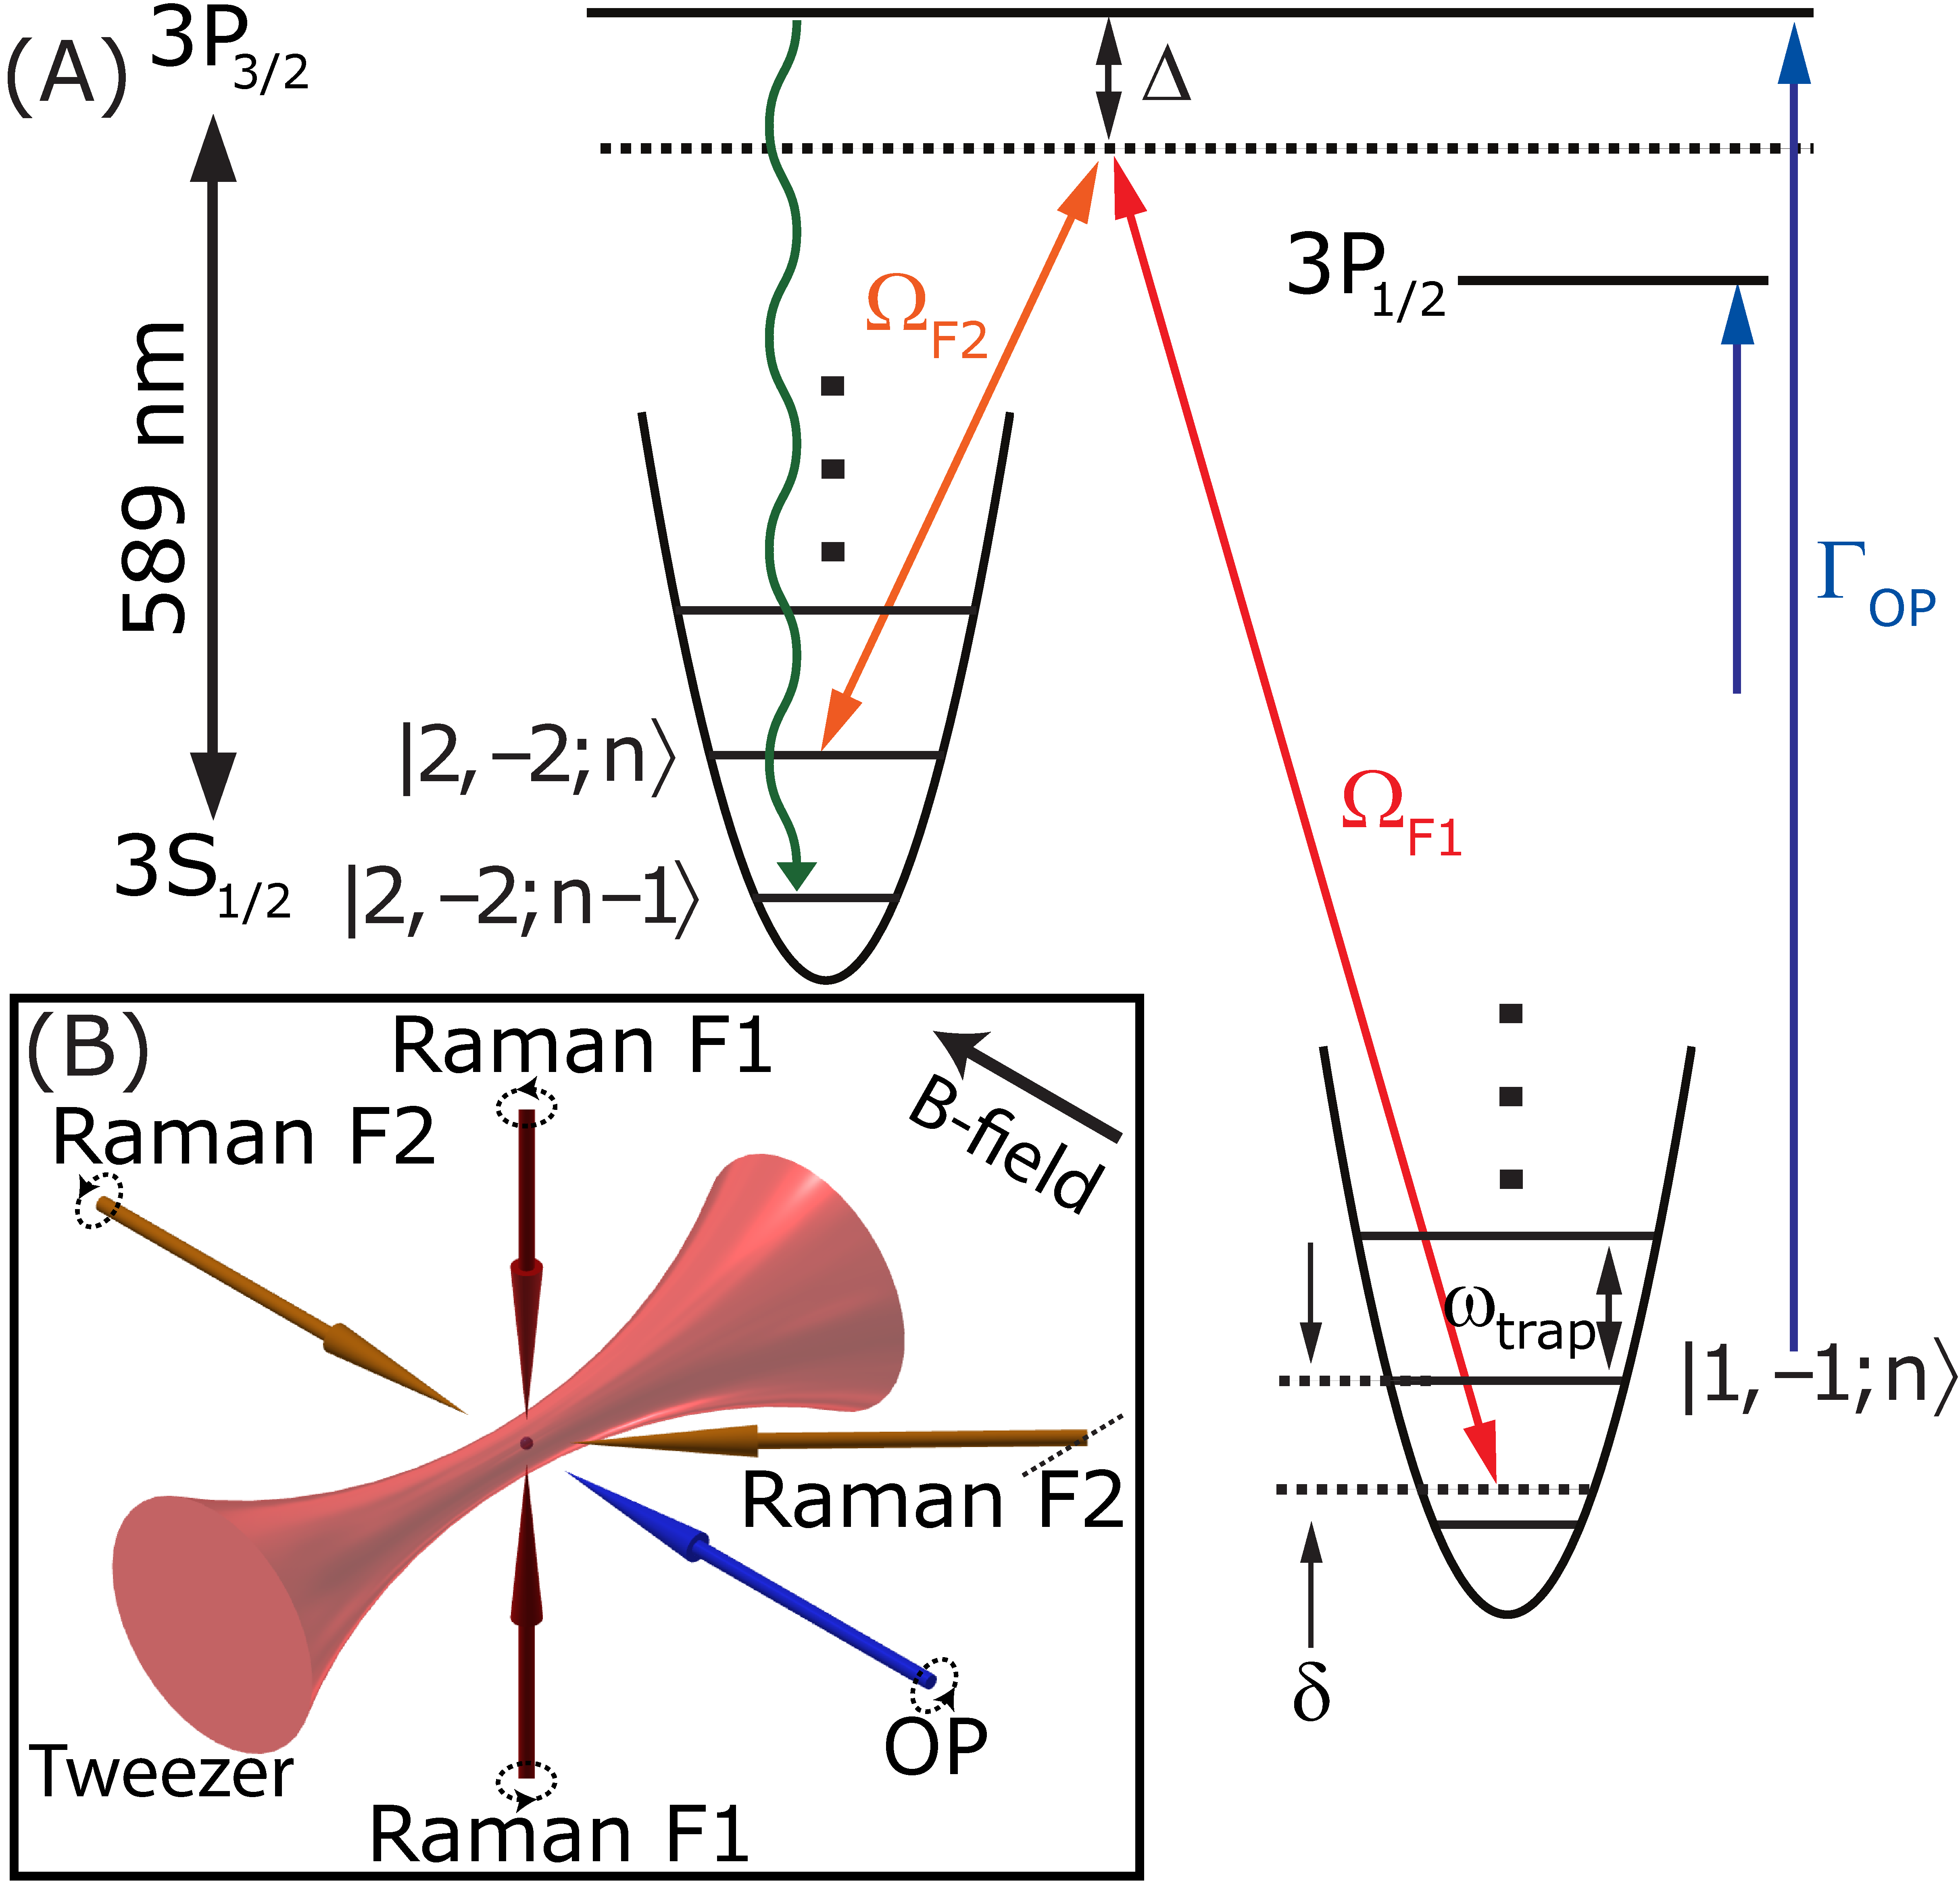
\includegraphics[height=7cm]{imgs/Na_RSC_schematic.pdf}
  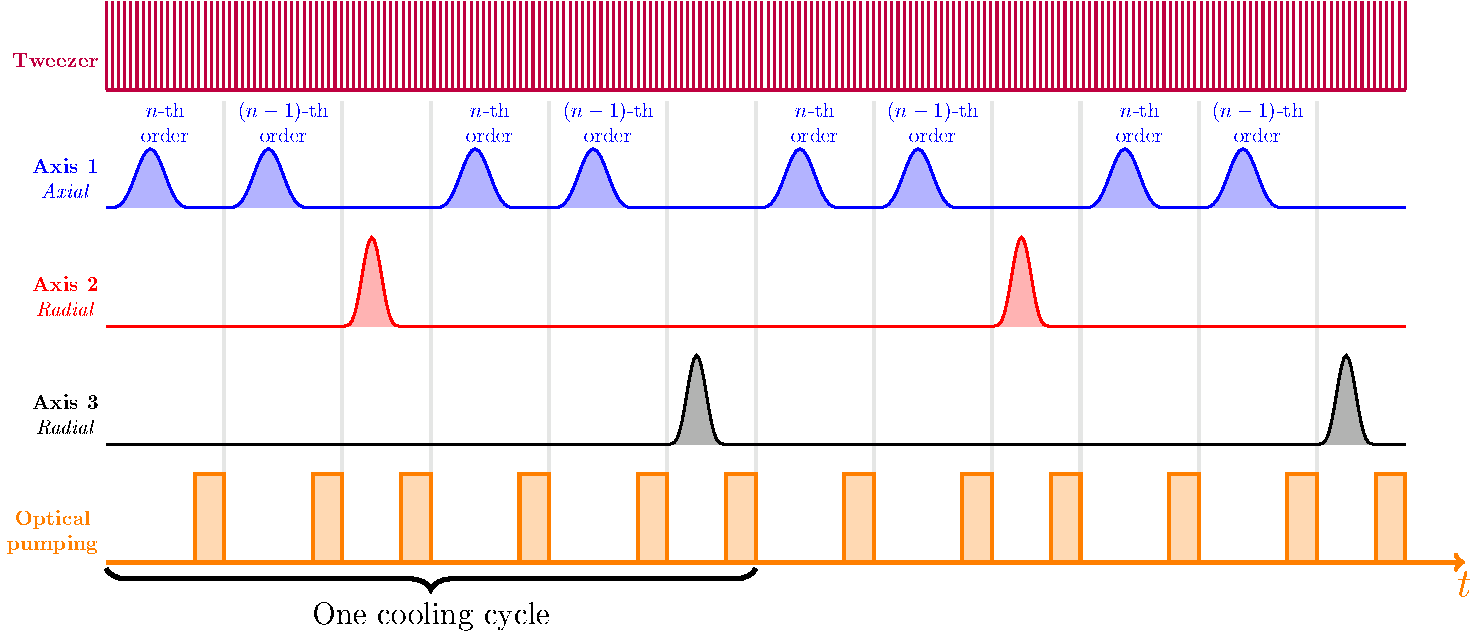
\includegraphics[height=7cm]{sequence.pdf}
  \caption{(A) Energy diagram. D1 OP
    (B) Beam diretions and polarizations
    (C) Sequence description
    \label{f-setup}}
\end{figure*}

We achieve the high ground state preparation fidelity needed for molecule formation
using Raman sideband cooling. The process consists of multiple cycles of laser pulses
to manipulate the internal and vibrational state of the atom.
Figure \ref{f-setup}A shows the schematic of the energy levels and the cooling sequence
in our setup.
Each cooling cycle starts with the Sodium atom in the $|F=2, m_F=-2\rangle$
ground electronic state and a certain vibration level $n$.
In the first step, a Raman pulse drives a transition on the motional sideband to lower
the vibrational state to $n-\Delta n$ while also changing the internal state
to $|F=1, m_F=-1\rangle$.
In the second step, which finishes the cooling cycle,
an optical pumping pulse bring the atom back to the $|F=2, m_F=-2\rangle$ state to take away
the entropy.
The geometry of the relavant beams and their polarizations is showed in figure \ref{f-setup}B.
The optical tweezer has one weakly confined axial direction (axis $1$) and
two more strongly confined radial directions (axis $2$ and $3$).
Multiple pairs of beams are used to drive the Raman transition during cooling in order to
isolate and maximize the coupling to different trap axis.

The optical pumping step may also change the vibrational level of the atom which
will cause heating. The possiblity for this to happen for an atom in the vibrational level $n$
is proportional to the effective Lamb-Dicke parameter $\eta^{eff}=\sqrt{n}\eta$ where $\eta=???$ is the Lamb-Dicke parameter.\\

Therefore, in order to perform Raman sideband cooling efficiently and minimize the heating during the optical pumping, we need to have a low initial temperature and a small Lamb-Dicke parameter. Comparing to previous realizations of Raman sideband cooling on heavier neutral alkali atoms like Rubidium[?] and Cesium[?], a few properties of Sodium makes this harder to achieve. Due to the unresolved(?) hyperfine structure in the $3^2P_{3/2}$ manifold, the sub-doppler cooling in Sodium is less efficient and we starts the Raman sideband cooling with a initial temperature of $40\mu K$, compare to $??\mu K$ for Cesium. Since the Lamb-Dicke parameter $\eta$ is inversely proportional to $\sqrt{m}$, it is also larger due for Sodium. With $45mW$ of power (??limited by trap switching??) at the focus of the trap, we measured a trapping frequency of $\{\omega_1,\omega_2,\omega_3\}/2\pi = \{67, 420, 580\} kHz$ which corresponds to an optical pumping Lamb-Dicke parameters of $\{\eta_{OP1},\eta_{OP2},\eta_{OP3}\} = \{???, ???, ???\}$. As a result, there is a very high probability of heating during the optical pumping step in the initial part of the cooling sequence.
This can be seen in figure [?], showing the probability distribution
of $n$ after optical pumping when the atom starts with different initial state. The probability
of staying in the same state drops very quickly as $n$ increases.\\

In additional to the high $\eta_{OP}$ for optical pumping, the Lamb-Dicke parameter for the Raman
transition $\eta_{Raman}$ is also very high on all three axis. For our geometry, we have $\{\eta_{Raman1},\eta_{Raman2},\eta_{Raman3}\} = \{???, ???, ???\}$.
The high $\eta_{Raman}$ means the sideband strength will not simple be proportional to $\sqrt{n}$ as it would be in the Lamb-Dicke regime. Instead, the sideband strength as a function of vibrational level $n$ in the axial direction is shown in figure [?].
Since the usual sideband thermometry, which measures $n/(n + 1)$ based on the ratio between heating and cooling sidebands, relies on the $\sqrt{n}$ scaling of the coupling strength, it breaks down
in our setup, making it harder to determing the temperature of the atom accurately. The strength
of the $-1$ order sideband also shows multiple points where the coupling strengh is very closed to
$0$, which means we cannot use this sideband to efficiently cool atom that is in those states.\\

Finally, the large number of populated vibrational level also means that the atom explores a larger percentage of the trap and is therefore more sensitive to trap anharmonicity.
This sets a lower limit on the minimum Raman Rabi frequency we can use in order to drive all
vibrational states efficiently.\\

% * Loose confinement
% ** More heating
% ** Complex sideband spectrum
% ** Matrix element minimum
% * Trap depth limit due to switching
% * High occupation
% ** Need more cooling
% ** Trap anharmonicity

\begin{figure}
  \includegraphics[width=9cm]{../../calculations/sideband_strength/imgs/coupling_0.46_0-6.png}
  \includegraphics[width=9cm]{../../calculations/sideband_strength/imgs/coupling_0.61_op-pi.png}
  \caption{(A) Matrix elements as a function of $n$ and $\Delta n$ (showing complex dependency and zeros) (B) State changing probability. Large and increases as $n$ gets larger
    \label{f-ld}}
\end{figure}

Fortunately, the features that make cooling Sodium challenging also provide us unique tools to
overcome these difficulties. As shown in figure [???], the high $\eta_{Raman}$ also causes the
coupling to higher order sideband during the Raman transition to be stronger,
especially for high vibrational states. This enables us to drive on high order Raman sidebands
to remove more vibrational energy in a single cooling pulse.
Since the heating from optical pumping is also worse for high vibrational states,
cooling on the high order sidebands can greately suppress the high heating during optical pumping.
The sideband strength for different orders are also oscillating out of phase, so we can generally
use a different sideband order to address vibrational states that cannot be efficiently addressed
by one sideband order.\\

% * Loose confinement
% ** Use higher orders to cool

Taking all the features of our system into account, we use a Monte-Carlo similation to verify
the validity of our method and explore the large parameter space for the cooling sequence.
In the simulation, we can observe the high heating rate due to the high Lamb-Dicke parameters
and confirm that high order of Raman sideband can be used to suppress this effect and reduces
the vibrational energy of the atom faster.
We also use the simulation to find a robust cooling strategy. As shown in figure (?),
we found that instead of cooling on only one sideband order at a time, it is generally more
efficient to alternate the cooling pulse between two neighboring orders. A cooling sequence
like this minimizes the accumulation of atom in a state not addressed by a particular sideband order.\\

\begin{figure*}
  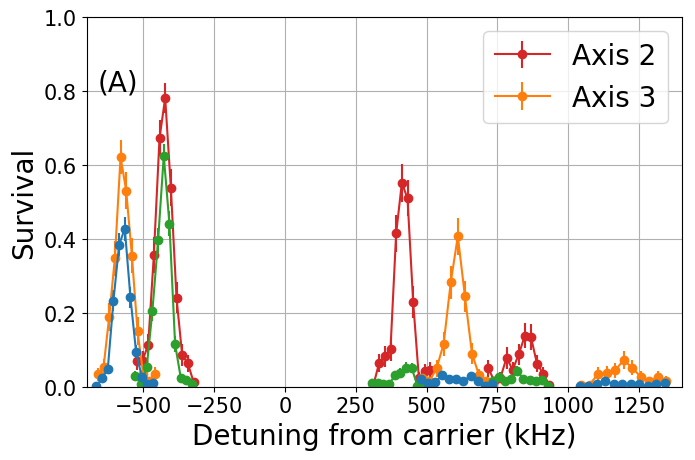
\includegraphics[width=8cm]{imgs/spectrum_r.png}
  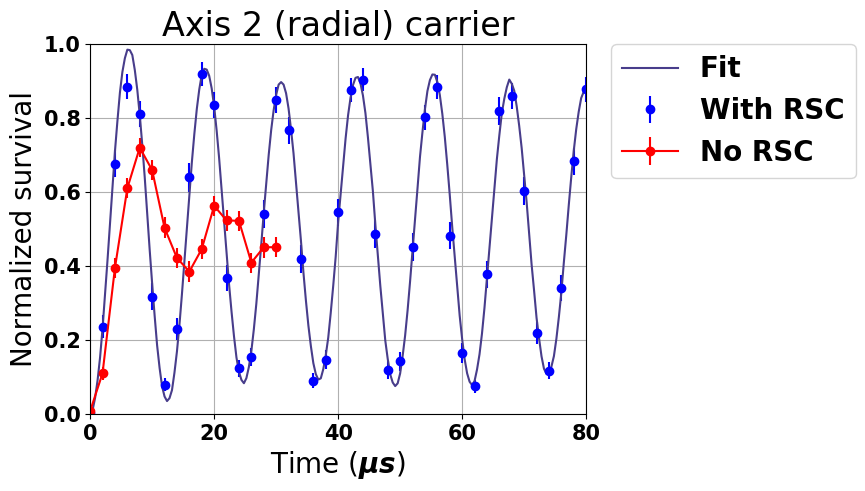
\includegraphics[width=8cm]{../../experiments/rabi_flop/imgs/fit_20170409_r2_0_ba.png}
  \caption{(A) (B) \label{f-radial}}
\end{figure*}

For the more tightly confined radial directions, we starts the cooling with $\{\bar n_2, \bar n_3\}=????, ????$. The sideband spectra of the initial distribution is shown in figure \ref{f-radial}A where we can clearly see the first order heating, first order cooling and second order cooling sidebands. After applying about 1000 cooling pulses cooling in all three dimentions starting with cooling on the radial second order, the Raman spectrum with the same parameter is shown in figure \ref{f-radial}B, where both cooling orders are suppressed. We can estimate the ground state probability in each direction based on the height of the first order cooling and heating sideband and the absence of the second order cooling sideband to be $......$. Due to the complexity of the sideband structure, we also use the Rabi flopping on the carrier and heating sideband as a independent measurement of the ground state population and gets $......$, showing good agreement between the two methods. (????? figure \ref{f-radial}C and \ref{f-radial}D)\\

\begin{figure*}
  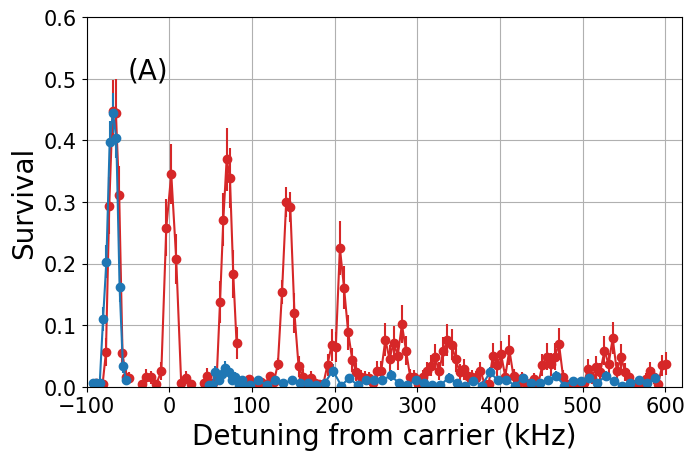
\includegraphics[width=8cm]{imgs/spectrum_a1.png}
  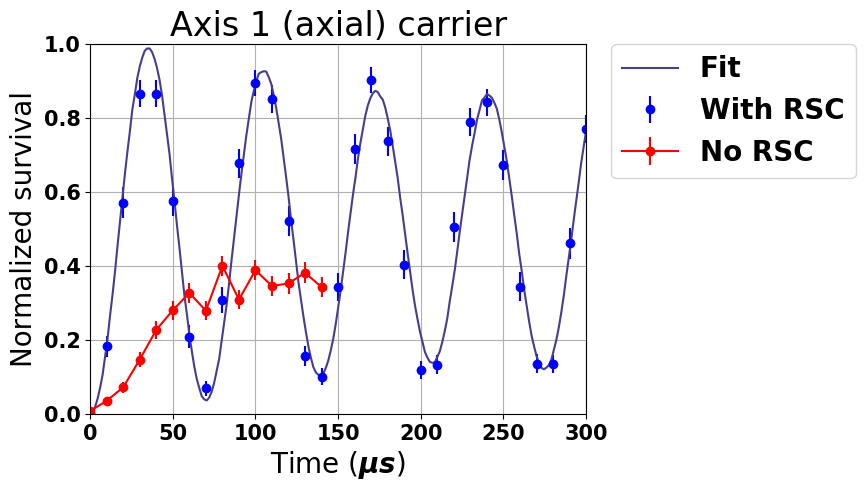
\includegraphics[width=8cm]{../../experiments/rabi_flop/imgs/fit_20170409_a1_0_ba.png}
  \caption{(A) (B) \label{f-axial}}
\end{figure*}

As mentioned previously, the axial direction is much less confined and therefore has a much higher
effective Lamb-Dicke parameter of $\sqrt{n}\eta_{Raman1}\approx2.4$. The Raman spectrum before applying Raman sideban cooling is shown in figure \ref{f-axial}A where we can see clearly resolved Raman cooling sidebands up to the 8th order suggesting that we have many vibrational states populated in this direction.\\

\ \\
\ \\
\ \\
\ \\
\ \\
\ \\
\ \\
\ \\
\ \\
\ \\
\ \\
\ \\
\ \\
\ \\
\ \\
\ \\
\ \\
\ \\
\ \\
\ \\
\ \\
\ \\
\ \\
\ \\
\ \\
\ \\
\ \\
\ \\
\ \\
\ \\
\ \\
\ \\
\ \\
\ \\
\ \\
\ \\
\ \\
\ \\
\ \\
\ \\
\ \\
\ \\
\ \\
\ \\
\ \\
\ \\
\ \\
\ \\
\ \\
\ \\
\ \\
\ \\
\ \\
\ \\
\ \\
\ \\
\ \\
\ \\
\ \\
\ \\
\ \\
\ \\
\ \\
\ \\
\ \\
\ \\
\ \\
\ \\
\ \\
\ \\
\ \\
\ \\
\ \\
\ \\
\ \\
\ \\
\ \\
\ \\
\ \\
\ \\
\ \\
\ \\
\ \\
\ \\
\ \\
\ \\
\ \\
\ \\
\ \\
\ \\
\ \\
\ \\
\ \\
\ \\
\ \\
\ \\
\ \\
\ \\

% Missing:
% ?? Switching helps OP fidelity
% ?? off-resonant scattering
% ?? D1 OP
% ?? Switching improves

\bibliography{paper}
\end{document}

% Generalization to other systems (properties that are shared with "more real" systems)
% Inharmonicity -> gaussian beam. -> importance to use short/strong pulses.
